%!TEX root = ../thesis.tex
\newchap{Statistical methods}\label{sec:STAT}
\minitoc
\section{Neural networks}
\subsection{Attention mechanism}

\section{Signal extraction}

\subsection{Likelihood construction}
The signal extraction procedure relies on a maximum likelihood fit of a binned distribution of one or more observables.\\
The likelihood is constructed as the product of Poisson distributions, one for each bin, that contains the parameter of interest (POI) to fit.\\
Given $C$ channels\footnote{A channel is defined by a set of cuts and selections that have the scope to isolate the signal and reject the background or viceversa}, each that contains $P_c$ processes, represented with histograms with $B_c$ bins, once we have the signal and the background MC predictions $s_{cb}$, $b_{cb}$, and the observed bin content $n_{cb}$ \footnote{Index $c$ stands for "channel", $p$ for "process", $b$ for "bin"}, the likelihood is \cite{Khachatryan2015PreciseTeV}
\begin{equation}
    \mathcal{L}(\mu)=\prod_c^C \prod_b^{B_c} \frac{(\mu s_{cb}+b_{cb})^{n_{cb}}}{n_{cb}!} e^{-(\mu s_{cb}+b_{cb})}
\end{equation}
In this case, the POI is the signal strength $\mu$, that is estimated by finding the value that maximizes the likelihood. The optimization problem is solved using the \textsc{MIGRAD} algorithm \cite{James1998MINUIT:Manual}, implemented in the \textsc{MINUIT2} library, that performs a line search in direction of the gradient and updates the covariance matrix (inverse of the Hessian matrix) with each step.\\
To improve the numerical stability, the software implementation exploits the negative log likelihood $\textit{NLL}=-\log{\mathcal{L}}$ instead of the likelihood in the form of the \Eq{eq:likelihood}  
\begin{equation*}
    \hat{\mu}=argmin_\mu - \log{\mathcal{L}(\mu)}
\end{equation*}
The predictions for each process are obtained through MC simulations, rescaled to match the total number of expected observed events. If $N^{MC}_{cp}$ is the total number of entries in the histogram relative to the process $p$ in the channel $c$, the respective entries have to be rescaled by a factor $w_{cp}$
\begin{equation}
    w_{cp}=\frac{\mathcal{L_I} \sigma_p \epsilon_{cp}}{N_{cp}}
\end{equation}
where $\mathcal{L_I}$ is the integrated luminosity, $\sigma_p$ the cross-section of the process $p$ and $\epsilon_{cp}$ the fraction of events of the process $p$ that pass the preselection defined by the channel $c$ that is estimated using MC events. 
\\
\paragraph*{Systematic uncertainties}
To incorporate in the model all the relevant uncertainties (\ie luminosity and rate uncertainties, uncertainties related to the detector resolution, etc.) we add to the likelihood the so-called nuisance parameters $\vec{\theta}$.\\
The likelihood becomes \cite{Conway2011IncorporatingSpectra}
\begin{equation}\label{eq:likelihood}
    \mathcal{L}(\mu,\vec{\theta})=\prod_c^C \prod_b^{B_c} Poiss \big( n_{cb}| \lambda_{cb}(\mu,\vec{\theta}) \big)  \prod_k  \pi_{k}(\theta_k)
\end{equation}
where $\pi_{k}$ is the prior probability distribution of the nuisance $\theta_k$.\\
The expectation value $\lambda_{cb}$ of the Poisson distribution now depends on the nuisance parameters that can be classified into normalization nuisances, shape nuisances and statistical nuisances.
\begin{equation}\label{eq:lambda}
     \lambda_{cb}( \mu,\vec{\theta})=\sum_p^{P_c}M_{cp}(\mu) N_{cp}(\vec{\theta}_n)y_{cpb}(\vec{\theta}_s)+E_{cb}(\vec{\theta}_{MC})
\end{equation}
The term $M_{cp}(\vec{\mu})$ is the physical model that contains the POI to fit, $N_{cp}(\vec{\theta_n})$ contains the factors relative to normalization nuisances, $y_{cpb}(\vec{\theta}_s)$ is the predicted content of each bin (that depends on shape nuisance parameters) and $E_{cpb}(\vec{\theta}_{MC})$ represents bin per bin the statistical error of the Monte Carlo predictions.\\
In the absence of systematic uncertainties, we have $N_{cp}=1$ and $E_{cb}=0 \quad \forall c,p,b$ and
$M_{cp}=\mu$ if $p$ is a signal process, otherwise $M_{cp}=1$; while $y_{cpb}$ is just the predicted bin content for each process.\\
All the nuisance parameters $\theta_k$ are defined in units of standard deviations\footnote{it means that $\theta=\pm 1$ correspond to a $\pm 1 \sigma$ variation.}.\\
Given that we know the central values and the standard deviations of all the variations, following the maximum entropy principle \cite{Jaynes2003ProbabilityScience}, we can use the normal distribution as a prior for all the nuisance parameters.
\begin{equation}
    \pi_k(\theta_k)=\mathcal{N}\left(\theta_k|0,1\right)=\frac{1}{\sqrt{2\pi}}e^{-\theta_k^2/2}
\end{equation}
\begin{itemize}
    \item \textbf{Normalization nuisances} are multiplicative corrections that affect the normalization of one process (\eg the cross-section uncertainties) or of all processes (\eg the luminosity uncertainties).\\
    This type of uncertainty does not change the shape of the histogram but changes the number of expected events.\\
    In $\lambda_{cb}$ [eq. \ref{eq:lambda}], they are represented by the term
    \begin{equation}
        N_{cp}\left(\vec{\theta}_n\right)=k_{cp}^{\theta^{(n)}_k}
    \end{equation}
    where $k_{cp}$ the relative $+1 \sigma$ variation from the nominal event yield for the process $p$ in the channel $c$ estimated through theory calculation of external measurements, while $\theta_{k}$ is the relative normalization nuisance parameter.\\
    \item \textbf{Shape nuisances}: Shape changing nuisances are produced by uncertainties
    that cause a different variation of event yields for each different bin.\\
    The model parameters are varied of $\pm 1 \sigma$ around their central value, creating an “Up” and a “Down” variation.\\
    The bin content $y_{cpb}$ has to be modified by multiplying a continuous and differentiable function of $\vec{\theta}_{s}$, so, given $\delta_b^\pm$ the differences between the $\pm 1 \sigma$ bin content variations of the bin and the nominal one, the up and down variations are interpolated with a spline in a procedure called "vertical morphing" \cite{Conway2011IncorporatingSpectra}
    \begin{equation}
    f_b\left(\theta_k^{(s)}\right)=
        \begin{cases}
            {\frac{1}{2}}\left((\delta_b^{+}-\delta_b^{-})\theta_k+{\frac{1}{8}}(\delta_b^{+}+\delta_b^{-})(3\theta_k^{6}-10\theta_k^{4}+15\theta_k^{2})\right) & \text{for } |\theta_k|\leq 1\\
            \theta_k \delta^+ & \text{for } \theta_k>1\\
            -\theta_k \delta^{-} & \text{for } \theta_k<-1
        \end{cases}
    \end{equation}
    The term $y_{cpb}(\vec{\theta}_s)$ is then defined as 
    \begin{equation}
        y_{cpb}(\theta_s)=max\left(0,y_{cpb}+\sum_k f_{cpb}\left(\theta_k^{(s)} \right)\right)
    \end{equation}
    In this way we can clip $y_{cpb}$ to 0 preventing the height of the bin to being negative.\\
    The vertical morphing procedure is shown and described in details in \Fig{fig:morphing}



    
    \item \textbf{MC statistical nuisances}: The MC events used to predict the expected signal and background yield in each bin are limited.\\
    To model the statistical MC uncertainties, we could add a nuisance parameter per bin per process, following the Barlow-Beeston approach \cite{Barlow1993FittingSamples}.\\
    But, if we have enough statistics in each bin, we can just use a nuisance parameter per bin that scales the sum of the processes yield, following the Barlow-Beeston lite approach \cite{Barlow1993FittingSamples}.\\
    The term $E_{cb}$ in $\lambda_{bc}$ is the term related to the statistical uncertainties is
    \begin{equation}
        E_{cb}(\vec{\theta}_{MC})=\theta_b\left(\sum_p \left(e_{cpb}N_{cp}(\vec{\theta}_n)M_{cp}(\mu)\right)^2 \right)^{1/2}
    \end{equation}
    where $N_{cp}$ and $M_{cp}$ are the normalization factor and the physical model defined before.
    $e_{cpb}$ is the Poissonian standard deviation of the b-th bin in the process p. Considering that the $\hat{\sigma}_{Poiss}=\sqrt{y_b}$ and that the bin height has to be rescaled to match the expected number of observed events, $e_{cpb}$ is
    \begin{equation}
        e_{cpb}=w_{cp} \sqrt{N_{cpb}^{MC}}   =\frac{\mathcal{L_I} \sigma_p \epsilon_{cp}}{N^{MC}_{cp}} \sqrt{N^{MC}_{cpb}}
    \end{equation}
    where $N_{cpb}$ is the number of MC events in the b-th bin.\\
    The term $E_{cb}$ scales, linearly with the nuisance parameter, the event yield of the bin with the root square sum of the Poisson uncertainties of each process.\\
\end{itemize}
\begin{figure}[h!]
    \centering
    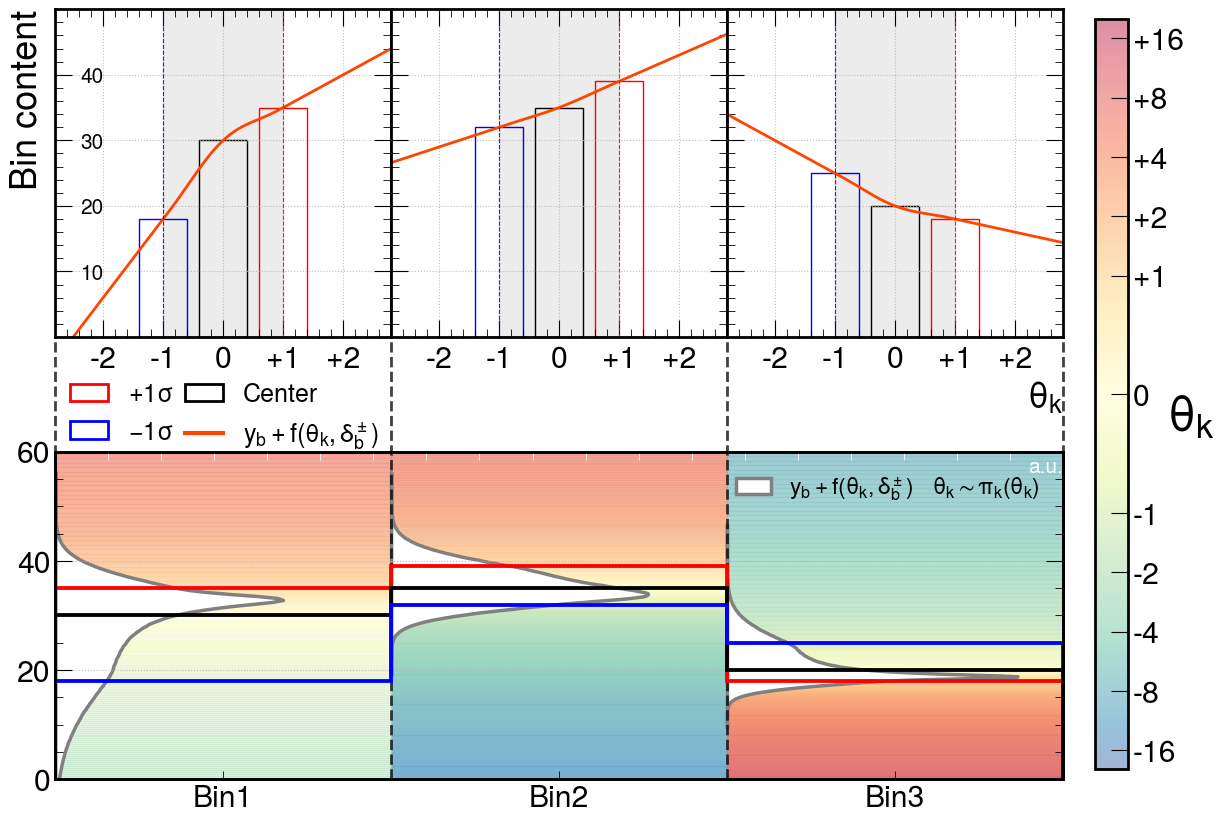
\includegraphics[width=\linewidth]{fig//chap05-stats/morphing.png}
    \caption{In the lower panel is represented an example of a histogram with 3 bins. The black line represents the histogram, the blue and the red lines represent the $\pm 1 \sigma$ shape variations.
    In the top panel, each bin is represented with its $\pm 1 \sigma$ variations and, on top of them, the $y_b+f(\theta_k,\delta_b^\pm)$ interpolation is shown with a red line. In the background of the lower panel, a color map shows, for each value of the bin height, the corresponding value of the nuisance parameter $\theta_k$, while the rotated vertical white shadow represents, for each bin, the probability distribution in arbitrary units of the expectation value of the Poisson distribution $\lambda_b=y_b+f(\theta_k,\delta_b^\pm)$ drawing $\theta_k$ from the normal prior.}
    \label{fig:morphing}
\end{figure}

\paragraph*{Smoothing}
For some systematics, up and down variations can lead to significant statistical fluctuations in the less populated bins, that, usually, are the high signal purity regions of the histogram.\\
To overcome this inconvenience, a smoothing procedure is applied.
\begin{algorithm}
\caption{Smoothing algorithm}\label{algo:smooth}
\begin{algorithmic}[1]
    \State Compute $r^{up}_b=y_{b}^{up}/y_b$ and $r^{down}_b=y_{b}^{down}/y_b$
    \State Compute $\delta r_b=\left(r^{up}_b-r^{down}_b\right)/2$
    \State Define $\hat{r}^{up}_b=1+\delta r_b$ and $\hat{r}^{down}_b=1+\delta r_b$
    \State Given $x_b$ is the position of the bin centers, apply the LOWESS smoothing algorithm to the points $(x_b,\hat{r}^{up}_b)$ and $(x_b,\hat{r}^{down}_b)$, finding the functions $f^{up}(x)$ and $f^{down}(x)$
    \State Redefine $y_b^{up}=y_b f^{up}(x_b)$ and $y_b^{down}=y_b f^{down}(x_b)$
\end{algorithmic}
\end{algorithm}
\\
The LOWESS algorithm \cite{Cleveland1979RobustScatterplots} (LOcally WEighted Scatterplot Smoothing) performs different linear regressions on a sliding window in different steps.


\begin{algorithm}
\caption{LOWESS algorithm}\label{algo:LOWESS}
\begin{algorithmic}[1]

    \State For each point $(x_i,y_i)$, create a window of a fixed length L.
    \State Define the weights $w_{1,ij}(x)=(1-|(x_j-x_i)/L|^3)^3 \; \Theta(L-|x_j-x_i|)$ where $\Theta$ is the Heaviside theta function.
    \State Perform a linear regression in each window, weighting each point with the defined weights $w_{1,ij}$. 
    \State Define $\hat{y}_i=f_{1,i}(x_i)$ where $f_{1,i}$ is the linear function obtained from the linear regression in each window.
    \State Compute the residuals $s_i=|y_i-\hat{y}_i|$.
    \State Normalize the residuals with $s_i=s_i/(6 m(s_i))$ where $m(s_i)$ is the median of the residuals.
    \State Define the weights $w_{2,i}=(1-s_i^2)^2 \; \Theta(1-s_i)$ 
    \State Perform a second linear regression on the points $(x_i,\hat{y}_i)$ weighting each point in the window with $w_{2,i}$, obtaining the functions $f_{2,i}$
    \State The smoothed curve is $(x_i,f_{2,i}(x_i))$

\end{algorithmic}
\end{algorithm}


\subsection{Profile Likelihood}
According to the Wilks' theorem \cite{James2006StatisticalEdition}, the distribution of the likelihood ratio is asymptotically distributed like a $\chi^2$.
\\
We have to fit just the POI $\mu$, so we can define the profile likelihood
\begin{equation}
    -2 \Delta \ln(\mathcal{L})=-2 \ln{\lambda(\mu)}= -2 \ln \left( \frac{\mathcal{L}(\mu,\bm{\tilde{\theta}}(\mu))}{\mathcal{L}(\hat{\mu}, \bm{\hat{\theta}})}\right) \sim \chi^2_1(\mu)
\end{equation}
$\hat{\mu}$ and $\bm{\hat{\theta}}$ are the parameters that maximize the likelihood simultaneously, while $\bm{\tilde{\theta}}(\mu)$ are the values of the nuisance parameters that maximize the likelihood for a fixed value of $\mu$.\\
Since $\int_0^1\chi^2_1(x) dx =0.683 = 1\sigma$, to compute the 68\% confidence level (CL) on $\hat{\mu}$, we can compute the profile likelihood and find the values of $\mu$ for which holds $-2\Delta \ln{\mathcal{L}(\mu)}=1$.\\
\\
To understand how different groups of nuisances affect the profile likelihood and the total uncertainty on $\mu$, some of the $\bm{\tilde{\theta}}(\mu)$ can be frozen in turn to the values $\bm{\hat{\theta}}$.\\
The so-called "breakdown procedure" consists in freezing sequentially groups of nuisance parameters, computing the profile likelihood and the relative uncertainties and subtracting them in quadrature from the total uncertainty.


\paragraph*{Impact plots} are a useful tool to understand the impact that each nuisance has on the total uncertainty. An example is shown in \Fig{fig:impact}.\\
\begin{itemize}
    \item In the left panel there are the names of the systematic sources, sorted according to their impact on the total uncertainty.
    \item In the center panel, there are two elements:
    \begin{itemize}
        \item[\ding{226}] The black bars ("Fit") represent the profile likelihood of the nuisance parameter. For each nuisance
        \begin{equation}
             \hat{\theta}_k=argmin_{\theta_k} -2 \ln \left( \frac{\mathcal{L}(\theta_k, \tilde{\mu}(\theta_k),\bm{\tilde{\theta}}(\theta_k))}{\mathcal{L}(\hat{\mu},\bm{\hat{\theta}},\hat{\theta}_k)} \right)
        \end{equation}
        is computed, along with the respective uncertainty, exploiting the Wilks' theorem as explained before.
        \item[\ding{226}] The blue crosses ("Pulls") corresponds to $(\hat{\theta}-\theta_{\text{pre-fit}})/\sqrt{\sigma_{\text{pre-fit}}^2-\sigma_{\text{post-fit}}^2}$.\\
        They tell us how much the fitted values are in tension with the pre-fit values defined by the priors.      
    \end{itemize}
    \item In the right panel there are the impacts.
    Once we have the fit for each nuisance, we can perform again the profile likelihood procedure on $\mu$ but fixing each nuisance in turn to their $\pm 1 \sigma_{\text{post-fit}}$ value. The blue and the red bars represent the values $\Delta^{\pm} \hat{\mu}=\hat{\mu}(\hat{\theta})-\hat{\mu}(\hat{\theta}_{\pm 1 \sigma})$.    
\end{itemize}
\begin{figure}[h!]
    \centering
    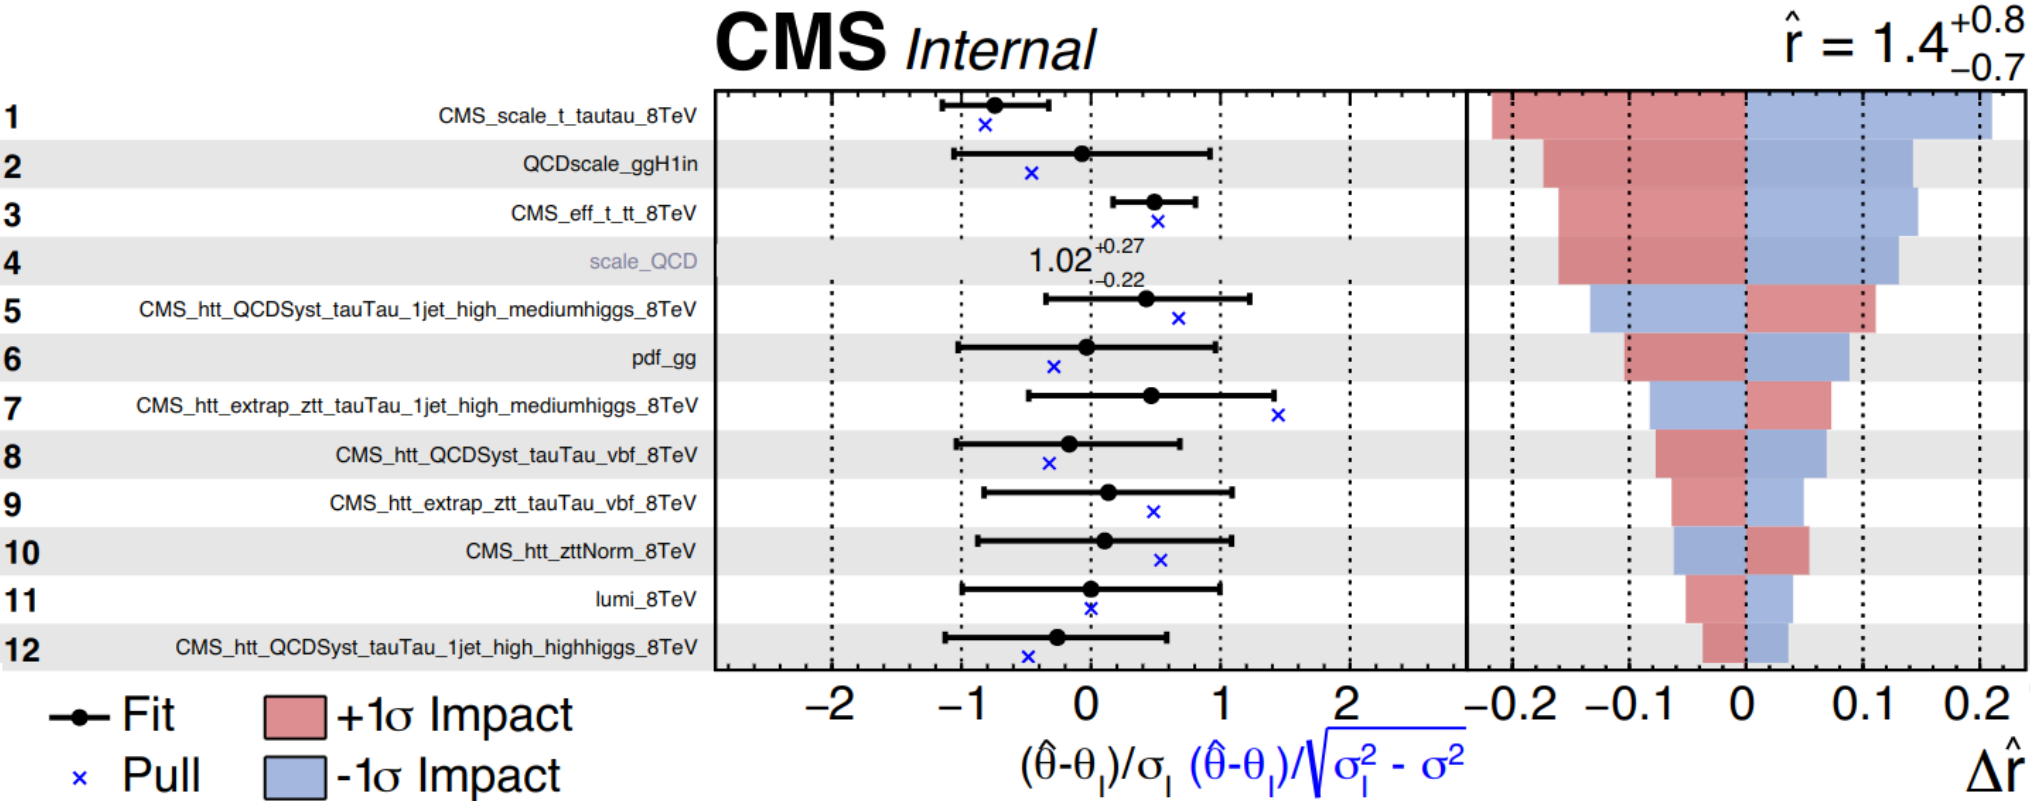
\includegraphics[width=1\linewidth]{fig/chap05-stats/impact.png}
    \caption{Example of an impact plot. In this plot, the POI $\mu$ is called $r$, and $\theta_I$, $\sigma_I$ are the pre-fit values.}
    \label{fig:impact}
\end{figure}


\subsection{Asimov dataset and significance} The term $n_{cb}$ in \Eq{eq:likelihood} is the number of observed events in the b-th bin, so, it contains real data.\\
To perform a simulation of an analysis, $n_{cb}$ can be replaced by MC events, creating the so-called "Asimov dataset" \cite{Cowan2011AsymptoticPhysics}
\begin{equation}
    n_{cb}^{\text{Asimov}}=\sum_p y_{cpb}
\end{equation}
In this way will be always $\hat{\mu}=1$ and $\bm{\hat{\theta}}=0$.\\
Using the Asimov dataset, the statistical uncertainties on $\hat{\mu}$ can be estimated through an approximation.
\begin{enumerate}
    \item Let's consider the Poisson log-likelihood for a single bin
\begin{equation}
    \ln\left(\mathcal{L}_b(\mu)\right)=n_b \ln(\mu s_b + b_b) - (\mu s_b + b_b)-\ln n_b! 
\end{equation}
and let's find the maximum likelihood estimator for $\mu$
\begin{equation}
    \partial_\mu \ln{\mathcal{L}_b}=0 \implies \hat{\mu}=\frac{n_b-b_b}{s_b}
\end{equation}
The variance of the estimator $\hat{\mu}_b$ is
\begin{equation}
    {\mathrm{Var}}(\hat{\mu}_b)=\frac{{\mathrm{Var}}(n_b)}{s_b^2}=\frac{\mu s_b + b_b }{s_b^2}
\end{equation}
The variance of $\hat{\mu}_b$ depends on $\mu$ itself, but, in the contest of the Asimov dataset, we can approximate it imposing $\mu=\hat{\mu}_b=1$, so the variance becomes
\begin{equation}
    {\mathrm{Var}}(\hat{\mu}_b)\sim \frac{s_b+b_b}{s_b^2}
\end{equation}
 \item The Cramer-Rao theorem \cite{James2006StatisticalEdition} states that, for a probability density function of the exponential family, to whom the Poisson distribution belongs, it holds
\begin{equation}
    \mathrm{Var}(\hat{\mu})=-\frac{(1-\partial_\mu b)^2}{E[\partial_\mu^2 \ln \mathcal{L}]}
\end{equation}
where $b$ is the bias of the estimator.
The maximum likelihood estimator is asymptotically unbiased, so we can neglect $b$.
\begin{equation}
    E[\partial_\mu^2 \ln \mathcal{L}_b]\sim-\frac{1}{\mathrm{Var}(\hat{\mu}_b)}
\end{equation}
and for the total likelihood
\begin{equation}
    E[\partial_\mu^2 \ln \mathcal{L}]=
    \sum_b E[\partial_\mu^2 \ln \mathcal{L}_b]=\sum_b
    -\frac{1}{\mathrm{Var}(\hat{\mu}_b)}
\end{equation}
but since it holds $\mathrm{Var}(\hat{\mu}) =-1/E[\partial_\mu^2 \ln \mathcal{L}]$, then
\begin{equation}
    \mathrm{Var}(\hat{\mu})=\left[\sum_b \frac{1}{\mathrm{Var}(\hat{\mu}_b)}\right]^{-1}= \left[\sum_b \frac{s_b^2}{s_b+b_b} \right]^{-1}
\end{equation}
\end{enumerate}
So, to estimate the uncertainty on $\hat{\mu}$ using the Asimov dataset, we can compute the so-called \textbf{significance}
\begin{equation}
    Q=\sum_c \sum_b \frac{s_{cb}^2}{s_{cb}+b_{cb}}
\end{equation}
and assert $\sigma(\hat{\mu}) \sim 1/\sqrt{Q}$
